\documentclass[reprint,amsmath,amssymb,aps,pra,nofootinbib,floatfix,showkeys]{revtex4-2}

\usepackage[utf8]{inputenc}
\usepackage[T1]{fontenc}
\usepackage[spanish,es-tabla,es-noquoting]{babel}
\usepackage{lmodern}
\usepackage{bm}
\usepackage{graphicx}
\usepackage{booktabs}
\usepackage{array}
\usepackage{mathtools}
\usepackage{xcolor}
\usepackage{microtype}
\usepackage{url}
\usepackage{hyperref}
\IfFileExists{siunitx.sty}{%
  \usepackage{siunitx}
  \sisetup{output-decimal-marker={,}, exponent-product=\cdot}
  \newcommand{\SIorNum}[2]{\SI{#1}{#2}}
}{%
  \newcommand{\num}[1]{##1}
  \newcommand{\SIorNum}[2]{##1\,\mathrm{##2}}
}

\graphicspath{{../../figures/}}
\hypersetup{
  hidelinks,
  pdftitle={ChaosLab: simulacion numerica del pendulo doble como sistema caotico de mecanica clasica},
  pdfauthor={Thomas Chisica},
  pdfsubject={Proyecto final de Fisica I},
  pdfkeywords={pendulo doble, caos, mecanica clasica, energia, ecuaciones diferenciales, simulacion numerica}
}

\newcommand{\dd}{\mathrm{d}}
\newcommand{\vect}[1]{\bm{#1}}
\newcommand{\Deltafase}{\Delta_{\mathrm{fase}}}

\begin{document}

\title{ChaosLab: simulaci\'on num\'erica del p\'endulo doble como sistema ca\'otico de mec\'anica cl\'asica}

\author{Thomas Chisica}
\affiliation{Curso F\'isica I, Escuela de Ciencias e Ingenier\'ia, Universidad del Rosario, Bogot\'a, Colombia}
\date{Socializaci\'on: viernes 29 de mayo, 11:00 a.m. a 1:00 p.m.}

\begin{abstract}
Este proyecto desarrolla una simulaci\'on computacional reproducible del p\'endulo doble para estudiar c\'omo un sistema mec\'anico cl\'asico puede pasar de un comportamiento regular a uno pr\'acticamente impredecible. El sistema se modela mediante dos coordenadas angulares, sus velocidades angulares y un conjunto de ecuaciones diferenciales ordinarias acopladas. La evoluci\'on temporal se integra con \texttt{solve\_ivp} usando el m\'etodo DOP853, y el resultado se eval\'ua con cuatro evidencias: trayectoria de las masas, conservaci\'on aproximada de la energ\'ia mec\'anica, divergencia de trayectorias casi id\'enticas y mapa de condiciones iniciales. Para el caso de referencia, una perturbaci\'on inicial de $10^{-6}\,\mathrm{rad}$ produce separaci\'on macrosc\'opica mientras la deriva relativa m\'axima de energ\'ia se mantiene en $2.56\times 10^{-6}$. Por tanto, la p\'erdida de predictibilidad observada no se interpreta como ausencia de leyes f\'isicas ni como falla num\'erica dominante, sino como consecuencia de la din\'amica no lineal del sistema.
\end{abstract}

\keywords{p\'endulo doble, caos cl\'asico, energ\'ia mec\'anica, ecuaciones diferenciales, integraci\'on num\'erica, visualizaci\'on cient\'ifica}

\maketitle

\section{Introducci\'on}

El p\'endulo simple es uno de los modelos b\'asicos de F\'isica I: una masa suspendida oscila bajo la acci\'on de la gravedad y, para \'angulos peque\~nos, se aproxima por movimiento arm\'onico simple. En ese modelo, la posici\'on se describe con un \'angulo $\theta$, la velocidad angular es $\omega=\dd\theta/\dd t$ y la aceleraci\'on angular es $\alpha=\dd^2\theta/\dd t^2$. La aproximaci\'on de Taylor
\begin{equation}
    \sin\theta \simeq \theta \qquad (|\theta|\ll 1)
    \label{eq:small-angle}
\end{equation}
linealiza la din\'amica y explica por qu\'e el periodo del p\'endulo simple se vuelve casi independiente de la amplitud.

El p\'endulo doble se obtiene al agregar una segunda barra y una segunda masa. La modificaci\'on parece menor, pero introduce dos grados de libertad, acoplamiento entre coordenadas y no linealidad. As\'i, el sistema sigue obedeciendo leyes deterministas de mec\'anica cl\'asica, pero su predicci\'on pr\'actica puede degradarse r\'apidamente. Esta tensi\'on entre determinismo y predictibilidad es una de las razones por las que el p\'endulo doble es un ejemplo cl\'asico de caos mec\'anico \cite{heyl2008double,rafat2009dynamics}.

La pregunta central del proyecto es: \emph{\textquestiondown c\'omo cambia la predictibilidad de un sistema mec\'anico al pasar de un p\'endulo simple a un p\'endulo doble, y c\'omo se evidencia esa sensibilidad mediante simulaci\'on num\'erica, conservaci\'on de energ\'ia y mapas de condiciones iniciales?}

\section{Objetivos}

El objetivo general es desarrollar una simulaci\'on computacional reproducible del p\'endulo doble, conectando mec\'anica cl\'asica, C\'alculo I, ecuaciones diferenciales y visualizaci\'on cient\'ifica para analizar trayectorias, energ\'ia mec\'anica, divergencia de condiciones iniciales y estructura global en el espacio de condiciones iniciales.

Los objetivos espec\'ificos son: implementar el modelo din\'amico como sistema de ecuaciones diferenciales ordinarias; resolverlo num\'ericamente y verificar conservaci\'on aproximada de energ\'ia; comparar trayectorias separadas por una perturbaci\'on microsc\'opica; construir un mapa de tiempo hasta el primer giro completo; y preparar una demostraci\'on interactiva que permita explorar par\'ametros del sistema.

\section{Modelo f\'isico}

\subsection{Coordenadas y estado}

Se consideran dos masas puntuales $m_1$ y $m_2$ unidas por barras ideales de longitudes $L_1$ y $L_2$. Los \'angulos $\theta_1$ y $\theta_2$ se miden desde la vertical hacia abajo. El estado de la simulaci\'on es
\begin{equation}
    \vect{s}(t)=
    \begin{bmatrix}
    \theta_1(t) & \omega_1(t) & \theta_2(t) & \omega_2(t)
    \end{bmatrix}^{\mathsf{T}},
    \label{eq:state}
\end{equation}
donde $\omega_i=\dd\theta_i/\dd t$. El problema se formula como un problema de valor inicial: dados $\vect{s}(0)$ y los par\'ametros f\'isicos, se integra $\dd\vect{s}/\dd t=\vect{f}(t,\vect{s})$.

\subsection{Posici\'on y energ\'ia}

Las posiciones cartesianas de las masas son
\begin{align}
    x_1 &= L_1\sin\theta_1, &
    y_1 &= -L_1\cos\theta_1, \\
    x_2 &= x_1+L_2\sin\theta_2, &
    y_2 &= y_1-L_2\cos\theta_2.
    \label{eq:positions}
\end{align}
De estas expresiones se obtiene la energ\'ia cin\'etica
\begin{align}
    T={}&\frac{1}{2}(m_1+m_2)L_1^2\omega_1^2
    +\frac{1}{2}m_2L_2^2\omega_2^2 \notag\\
    &+m_2L_1L_2\omega_1\omega_2\cos(\theta_1-\theta_2),
    \label{eq:kinetic}
\end{align}
y la energ\'ia potencial gravitacional
\begin{equation}
    V=-(m_1+m_2)gL_1\cos\theta_1-m_2gL_2\cos\theta_2.
    \label{eq:potential}
\end{equation}
La energ\'ia mec\'anica total es
\begin{equation}
    E(t)=T(t)+V(t).
    \label{eq:total-energy}
\end{equation}
En el modelo ideal, sin fricci\'on ni resistencia del aire, $E(t)$ debe conservarse. Por eso la deriva relativa
\begin{equation}
    \varepsilon_E(t)=\frac{|E(t)-E(0)|}{|E(0)|}
    \label{eq:energy-drift}
\end{equation}
se usa como prueba de calidad num\'erica.

\subsection{Sensibilidad a condiciones iniciales}

Para evidenciar sensibilidad se integran dos trayectorias con estados iniciales casi id\'enticos:
\begin{equation}
    \theta_2'(0)=\theta_2(0)+\epsilon,
    \qquad \epsilon=10^{-6}\,\mathrm{rad}.
    \label{eq:perturbation}
\end{equation}
La separaci\'on se mide en espacio de fases con diferencias angulares envueltas en $[-\pi,\pi]$:
\begin{equation}
    \Deltafase(t)=
    \sqrt{
    \delta\theta_1^2+
    \delta\theta_2^2+
    \delta\omega_1^2+
    \delta\omega_2^2 }.
    \label{eq:phase-distance}
\end{equation}
La pendiente temprana de $\log\Deltafase(t)$ frente a $t$ se reporta como indicador de divergencia inicial. No se afirma que esta pendiente sea un exponente de Lyapunov formal; se usa como medida cuantitativa apropiada para una demostraci\'on de F\'isica I.

\section{Metodolog\'ia computacional}

La simulaci\'on se implement\'o en Python. El sistema de ecuaciones diferenciales se integr\'o con \texttt{scipy.integrate.solve\_ivp}, funci\'on dise\~nada para resolver problemas de valor inicial de sistemas de ecuaciones diferenciales ordinarias \cite{scipy_solve_ivp}. Se us\'o el m\'etodo DOP853, con tolerancia relativa $10^{-9}$ y tolerancia absoluta $10^{-11}$.

Los par\'ametros de referencia fueron $m_1=m_2=\SIorNum{1}{kg}$, $L_1=L_2=\SIorNum{1}{m}$ y $g=9.81\,\mathrm{m\,s^{-2}}$. La condici\'on inicial principal fue
\begin{equation}
    \vect{s}(0)=
    \begin{bmatrix}
    120^\circ & 0 & -10^\circ & 0
    \end{bmatrix}^{\mathsf{T}}.
    \label{eq:initial-condition}
\end{equation}
Se generaron posiciones, energ\'ias y distancias de fase para producir las figuras principales.

El mapa de condiciones iniciales se calcul\'o como una colecci\'on de experimentos num\'ericos. Para cada punto $(\theta_1(0),\theta_2(0))\in[-\pi,\pi]^2$, con $\omega_1(0)=\omega_2(0)=0$, se integr\'o el sistema con RK4 vectorizado y se registr\'o el tiempo hasta el primer \emph{flip}, definido como el primer instante en que $|\theta_1|$ o $|\theta_2|$ alcanza $\pi$. Esta visualizaci\'on sigue la idea de mapas de condiciones iniciales usados para estudiar estructura fractal en p\'endulos dobles \cite{heyl2008double,reusser_double_pendulum}.

\begin{table}[b]
\caption{M\'etricas principales del experimento num\'erico de referencia.}
\label{tab:metrics}
\begin{ruledtabular}
\begin{tabular}{lc}
Magnitud & Valor \\
\hline
Perturbaci\'on inicial $\epsilon$ & $1.0\times10^{-6}\,\mathrm{rad}$ \\
Pendiente de $\log\Deltafase(t)$, $1$--$7\,\mathrm{s}$ & $1.09593\,\mathrm{s^{-1}}$ \\
Deriva relativa m\'axima de energ\'ia & $2.56083\times10^{-6}$ \\
Tiempo total de simulaci\'on del caso base & $24\,\mathrm{s}$ \\
\end{tabular}
\end{ruledtabular}
\end{table}

\section{Resultados}

\subsection{Trayectoria de la segunda masa}

La Fig.~\ref{fig:trajectory} muestra la trayectoria de la segunda masa. Aunque el sistema obedece ecuaciones deterministas, el movimiento resultante no se reduce a una oscilaci\'on peri\'odica simple. La curva exhibe orden local, porque cada punto se obtiene de leyes mec\'anicas precisas, pero tambi\'en estructura global compleja.

\begin{figure}[t]
    \centering
    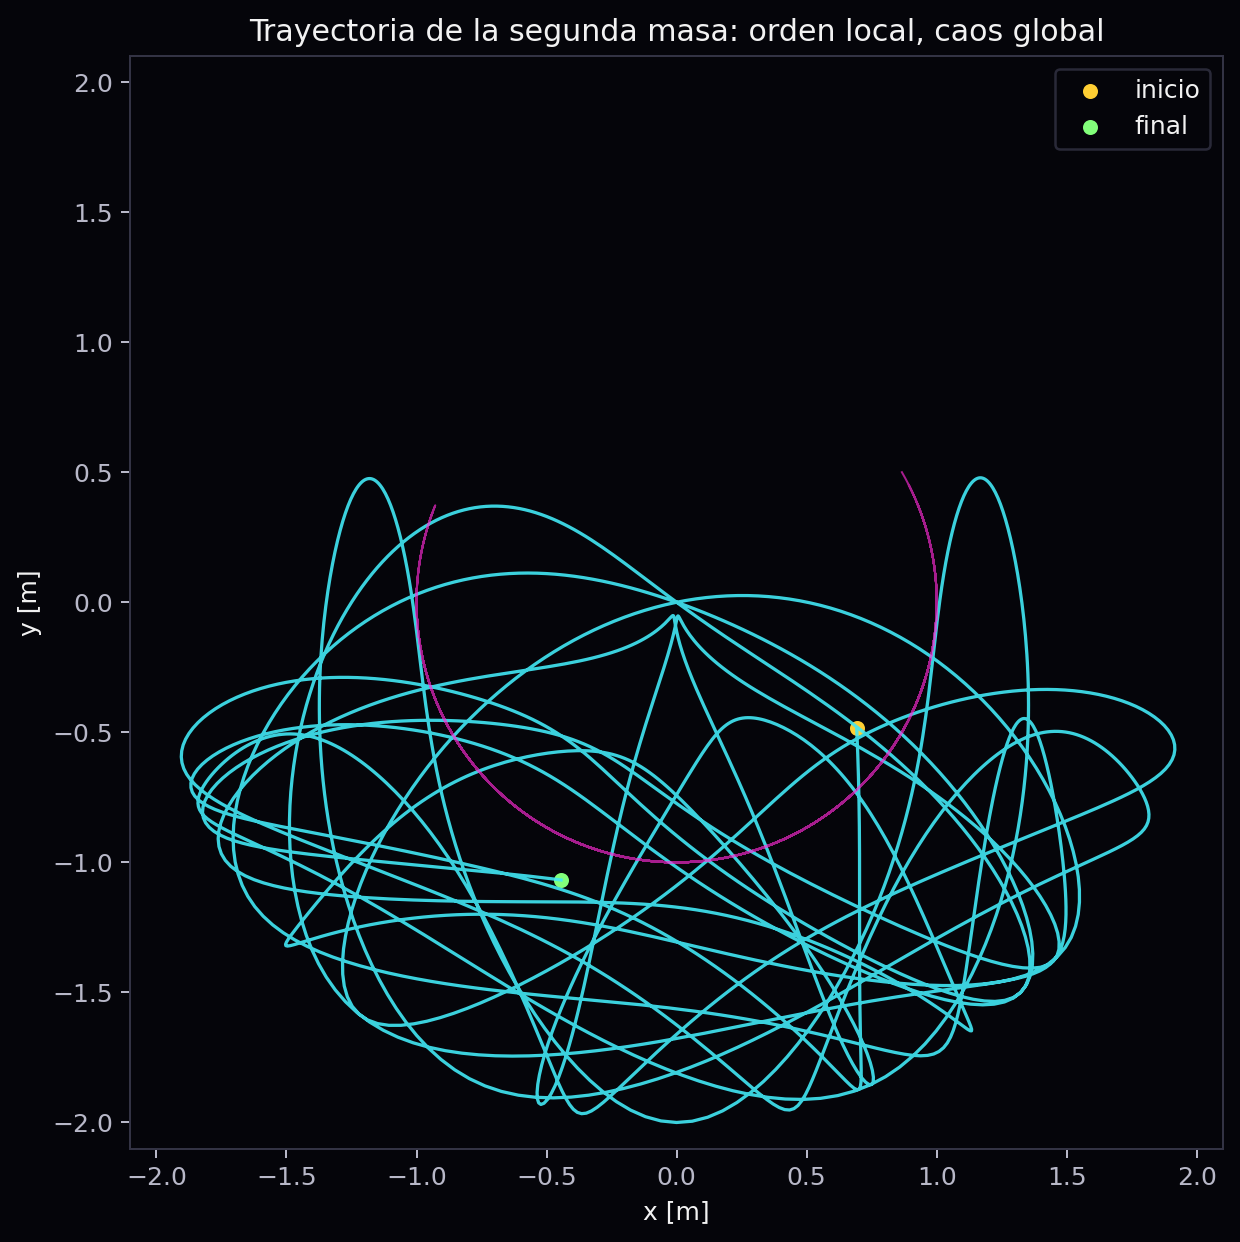
\includegraphics[width=\columnwidth]{trajectory_mass2.png}
    \caption{Trayectoria de la segunda masa para la condici\'on inicial de referencia. La curva ilustra c\'omo una regla mec\'anica determinista puede producir movimiento geom\'etricamente complejo.}
    \label{fig:trajectory}
\end{figure}

\subsection{Conservaci\'on de energ\'ia}

La Fig.~\ref{fig:energy} compara energ\'ia cin\'etica, potencial y total. La energ\'ia cin\'etica y la potencial intercambian magnitud durante el movimiento, mientras que la energ\'ia total permanece casi constante. Esto es esencial: antes de atribuir divergencia a caos, se debe verificar que el integrador no est\'e introduciendo una variaci\'on artificial grande en $E(t)$.

\begin{figure}[t]
    \centering
    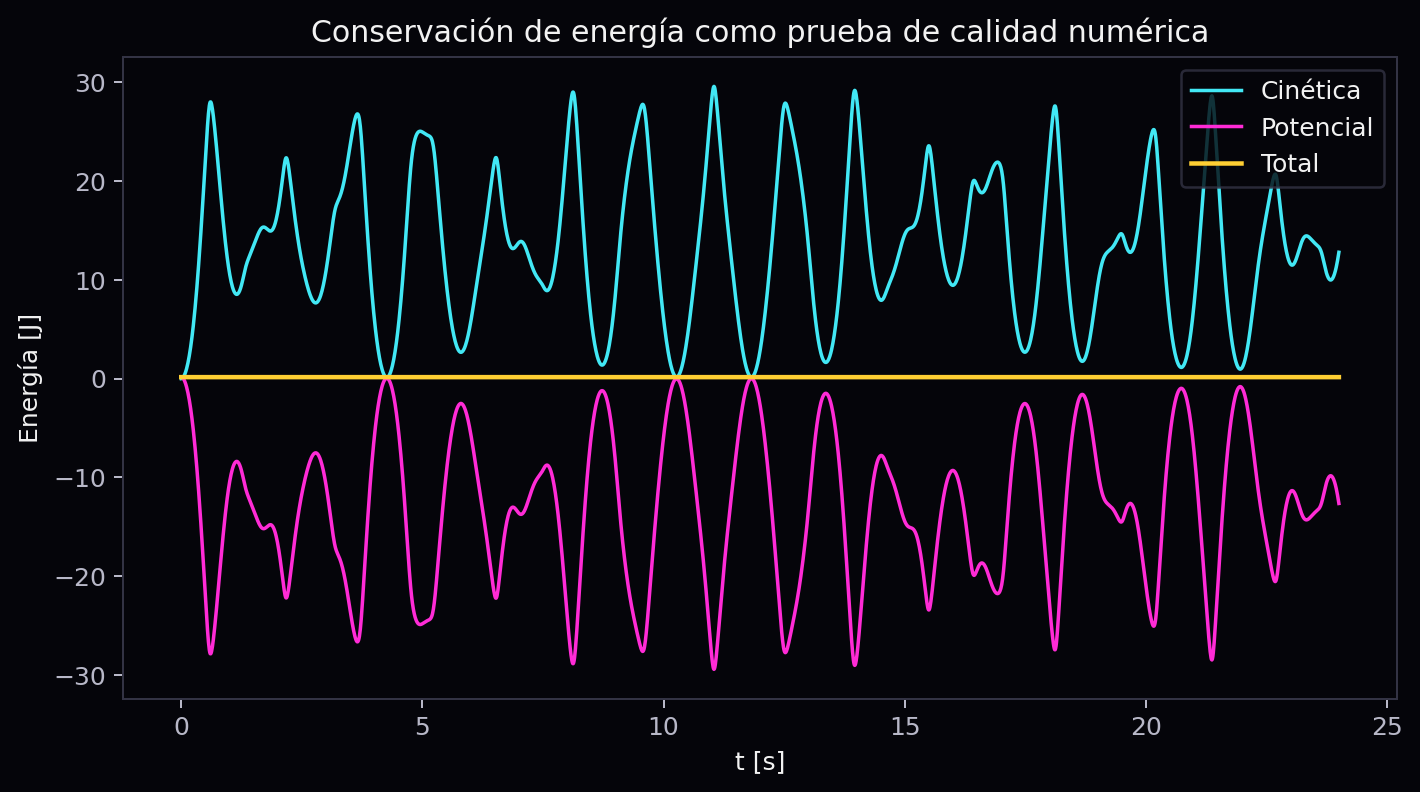
\includegraphics[width=\columnwidth]{energy_vs_time.png}
    \caption{Energ\'ia cin\'etica, potencial y total como funci\'on del tiempo. La conservaci\'on aproximada de $E=T+V$ funciona como control de calidad num\'erica.}
    \label{fig:energy}
\end{figure}

La deriva relativa m\'axima obtenida fue $2.56\times10^{-6}$, valor peque\~no para una simulaci\'on visual de este alcance. Por tanto, la divergencia entre trayectorias no se explica principalmente por una p\'erdida artificial de energ\'ia.

\subsection{Divergencia entre trayectorias}

La Fig.~\ref{fig:divergence} muestra $\Deltafase(t)$ en escala semilogar\'itmica. Al inicio, la separaci\'on es del orden de la perturbaci\'on impuesta. Despu\'es, la distancia crece varios \'ordenes de magnitud hasta que las trayectorias dejan de ser visualmente indistinguibles. Este resultado resume la idea central del proyecto: el sistema no es aleatorio, pero la predicci\'on pr\'actica se vuelve limitada porque peque\~nas diferencias iniciales se amplifican.

\begin{figure}[t]
    \centering
    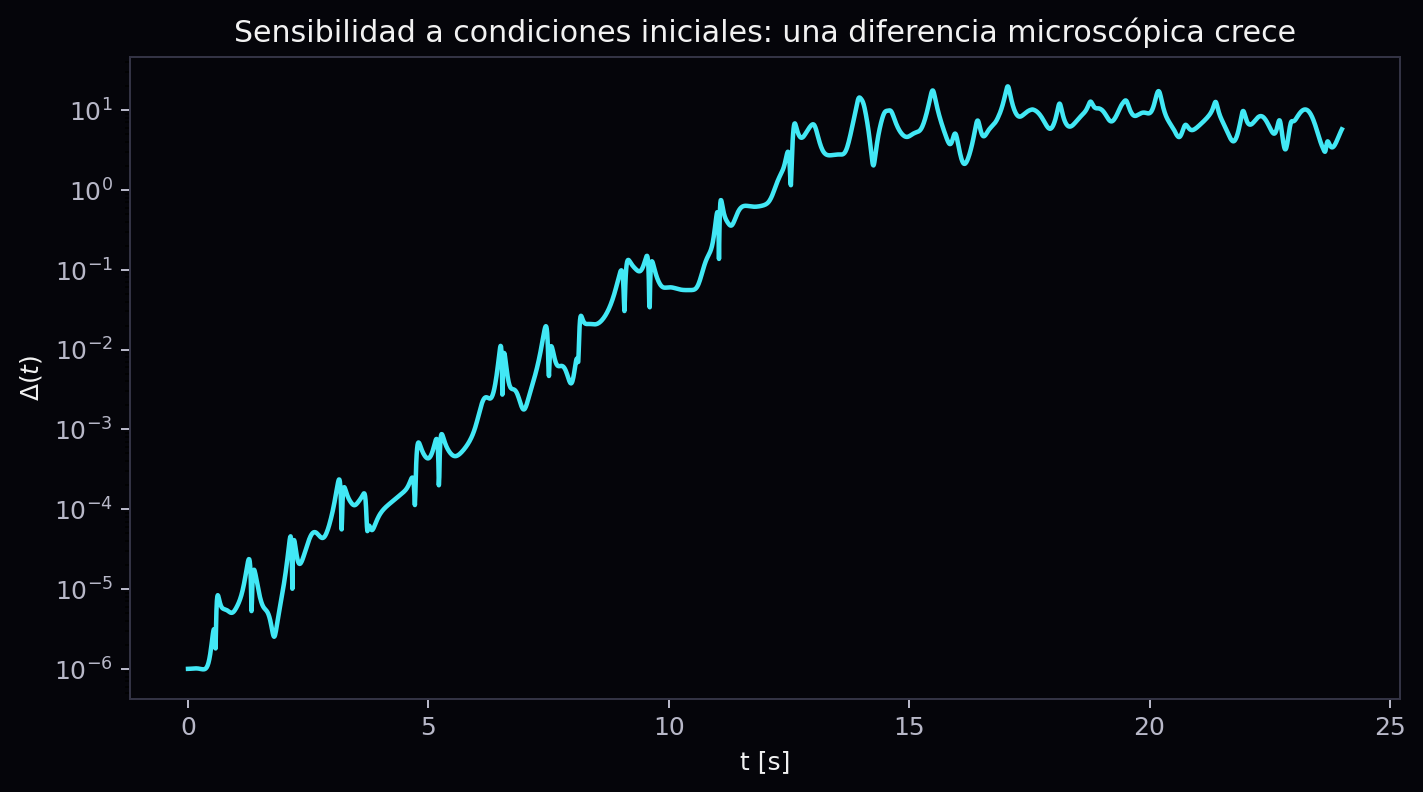
\includegraphics[width=\columnwidth]{divergence_semilog.png}
    \caption{Separaci\'on en espacio de fases entre dos trayectorias que difieren inicialmente en $10^{-6}\,\mathrm{rad}$. La escala logar\'itmica evidencia crecimiento temprano de la perturbaci\'on.}
    \label{fig:divergence}
\end{figure}

\subsection{Mapa de condiciones iniciales}

La Fig.~\ref{fig:map} condensa miles de simulaciones en una sola imagen. Cada pixel representa un par de \'angulos iniciales y el color indica el tiempo hasta el primer giro completo. Las regiones oscuras corresponden a condiciones que no hicieron \emph{flip} dentro de la ventana de simulaci\'on. Las fronteras entre regiones son altamente irregulares: un cambio peque\~no en los \'angulos iniciales puede cambiar de manera dr\'astica el resultado.

\begin{figure*}[t]
    \centering
    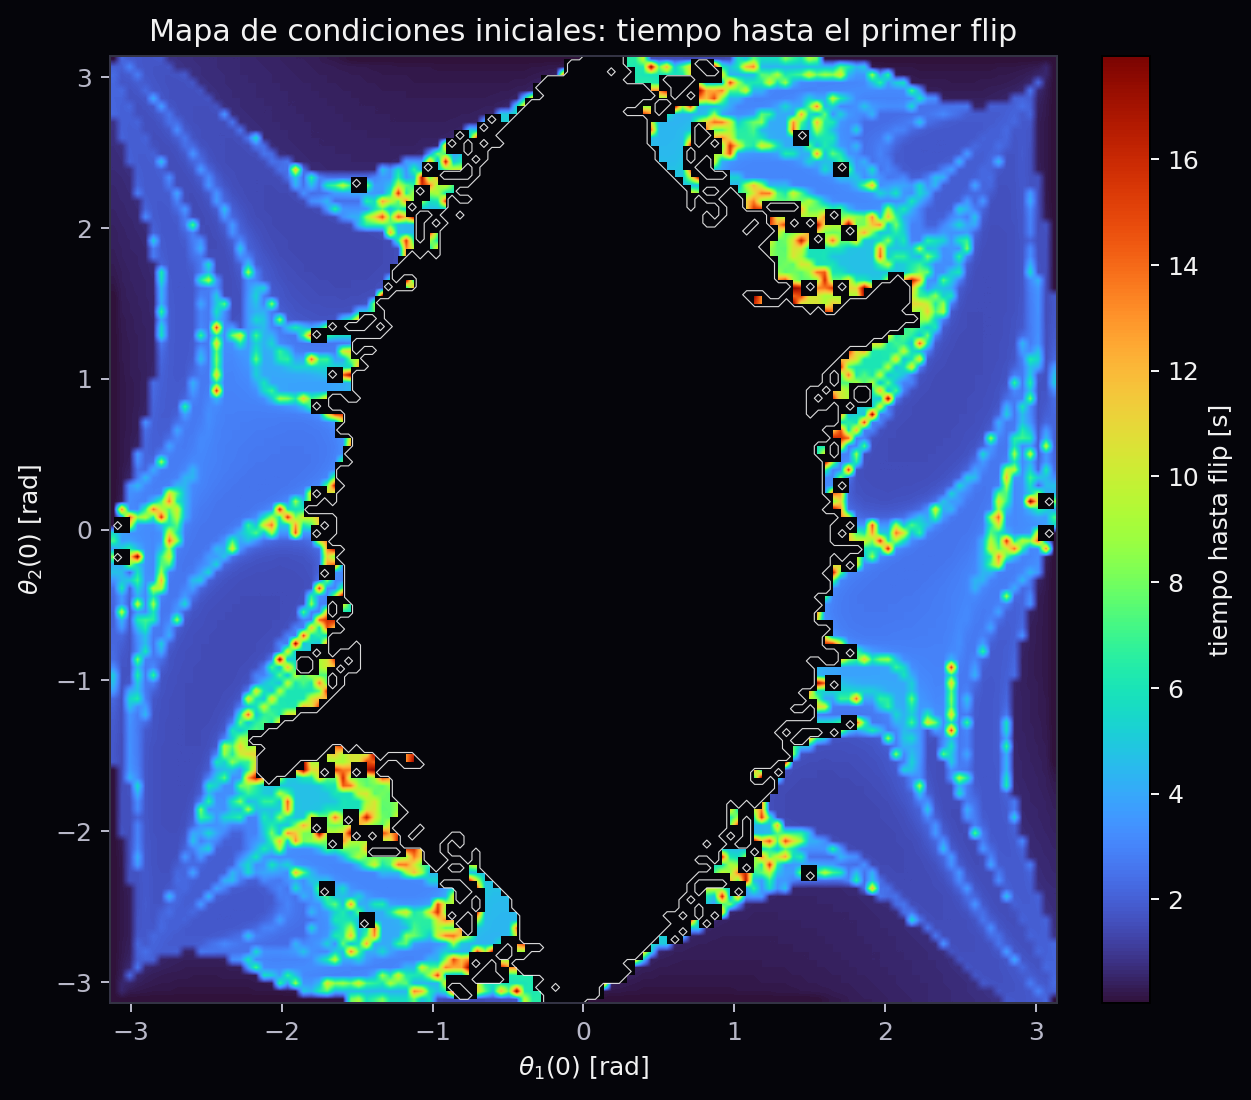
\includegraphics[width=0.70\textwidth]{flip_time_fractal_map.png}
    \caption{Mapa de condiciones iniciales. Cada pixel corresponde a un experimento num\'erico con $\omega_1(0)=\omega_2(0)=0$; el color representa el tiempo hasta el primer \emph{flip}.}
    \label{fig:map}
\end{figure*}

\section{Discusi\'on}

El resultado m\'as importante no es que el p\'endulo doble ``se vea complicado'', sino que esa complejidad aparece mientras se conserva aproximadamente la energ\'ia. Si la energ\'ia total variara de forma grande, la divergencia podr\'ia atribuirse a un error num\'erico dominante. En cambio, la simulaci\'on conserva $E(t)$ con deriva relativa del orden de $10^{-6}$, al tiempo que dos trayectorias separadas por $10^{-6}\,\mathrm{rad}$ divergen de manera visible.

El proyecto tambi\'en conecta directamente con C\'alculo I. Las velocidades y aceleraciones angulares son derivadas temporales; la aproximaci\'on de \'angulo peque\~no proviene de Taylor; la integraci\'on num\'erica acumula cambios locales para reconstruir la evoluci\'on global; y la pendiente de $\log\Deltafase(t)$ se interpreta como una tasa temprana de crecimiento. La visualizaci\'on no reemplaza la teor\'ia: la hace observable.

Finalmente, el mapa de condiciones iniciales muestra que el espacio de par\'ametros no est\'a dividido por fronteras simples. Esta observaci\'on es valiosa para la presentaci\'on oral porque transforma una pregunta abstracta, ``\textquestiondown qu\'e es sensibilidad a condiciones iniciales?'', en una imagen concreta: cada pixel obedece las mismas leyes, pero peque\~nas variaciones cambian el futuro del sistema.

\section{Limitaciones y trabajo futuro}

El modelo usa masas puntuales, barras ideales y ausencia de rozamiento. Por eso no pretende reproducir indefinidamente un p\'endulo doble real. Una validaci\'on experimental razonable consistir\'ia en construir un p\'endulo doble casero, grabar los primeros segundos y extraer posiciones con Tracker \cite{tracker_video}. La validaci\'on debe ser de corto plazo, porque la sensibilidad a condiciones iniciales amplifica errores de medici\'on.

El mapa de condiciones iniciales usa RK4 de paso fijo para obtener una imagen r\'apida y reproducible; por tanto, se interpreta como visualizaci\'on exploratoria, no como c\'alculo certificado de fronteras fractales. Como extensi\'on computacional podr\'ia entrenarse un modelo \emph{surrogate} para clasificar si una condici\'on inicial har\'a \emph{flip} antes de cierto tiempo, pero ese componente debe permanecer secundario. El n\'ucleo del proyecto es f\'isico: energ\'ia, no linealidad, ecuaciones diferenciales y sensibilidad.

\section{Conclusiones}

ChaosLab muestra que el p\'endulo doble es una extensi\'on natural y poderosa de los conceptos de F\'isica I. Al pasar del p\'endulo simple a dos grados de libertad, aparecen ecuaciones acopladas, transferencia de energ\'ia y sensibilidad extrema a condiciones iniciales. La simulaci\'on conserva la energ\'ia mec\'anica con deriva peque\~na, de modo que la divergencia observada no se debe principalmente a una falla num\'erica. El mapa de condiciones iniciales refuerza la tesis central: un sistema puede ser determinista y, aun as\'i, dif\'icil de predecir en la pr\'actica.

El resultado final es reproducible y defendible como proyecto de portafolio: combina mec\'anica cl\'asica, C\'alculo I, integraci\'on de ecuaciones diferenciales, visualizaci\'on cient\'ifica y una presentaci\'on interactiva inspirada en divulgaci\'on matem\'atica de alta calidad \cite{twoswap_swaptube}.

\bibliographystyle{apsrev4-2}
\bibliography{references}

\end{document}
